\section{动态环境下的SLAM系统}
\subsection{基于运动分割的SLAM技术}
\label{subsec:motion_segmentation}
动态分割(又称为移动物体检测/分割\cite{Derome2015Moving, Klappstein2008Moving, kundu2009movingA})透过将特征区分为两类特征,静态和动态特征,以检测图像中移动的区块。
明确地说,给定在图像空间中的特征点集合,动态分割将特征点聚类为静态集合和动态集合。
传统的视觉SLAM使用鲁棒的静态方法,计算几何模型(如基本矩阵、单应矩阵)来实现动态分割。
比如利用随机抽样一致算法(RANSAC)\cite{fischler1981randomA}和特定的距离度量方法(如桑普森距离\cite{Hartley2008Multiple})将不服从模型的点剔除。
当静态的特征点占了主体时,这种方法能够有很好的效果。
当动态物体占了相机的绝大部份, 或是捕捉到的场景被巨大的移动物体遮挡时,这种方法可能就会失败。
其他方法结合其他传感器来解决这个问题,如使用惯性测量单元(IMU)估计相机自身的运动\cite{Jones2011Visual, Leutenegger2014Keyframe}。
通过IMU得到的位姿估计可以用来初始化相机位姿并且鲁棒地分割静态和动态特征。
在这一章节,我们讨论传统视觉SLAM和视觉惯性SLAM之外,分割静态和动态物体的其他方法。

\subsection{背景--前景初始化}
背景-前景初始化技术假设系统有对于环境的先验知识,利用这个信息分割静态和动态特征。这个先验知识可以归于背景( 静态特征)或是前景( 动态特征)。
如果系统的先验知识是关于前景目标,表示系统知道相机前方运动物体的类型或形状。

\begin{figure}[thbp]
	\centering
	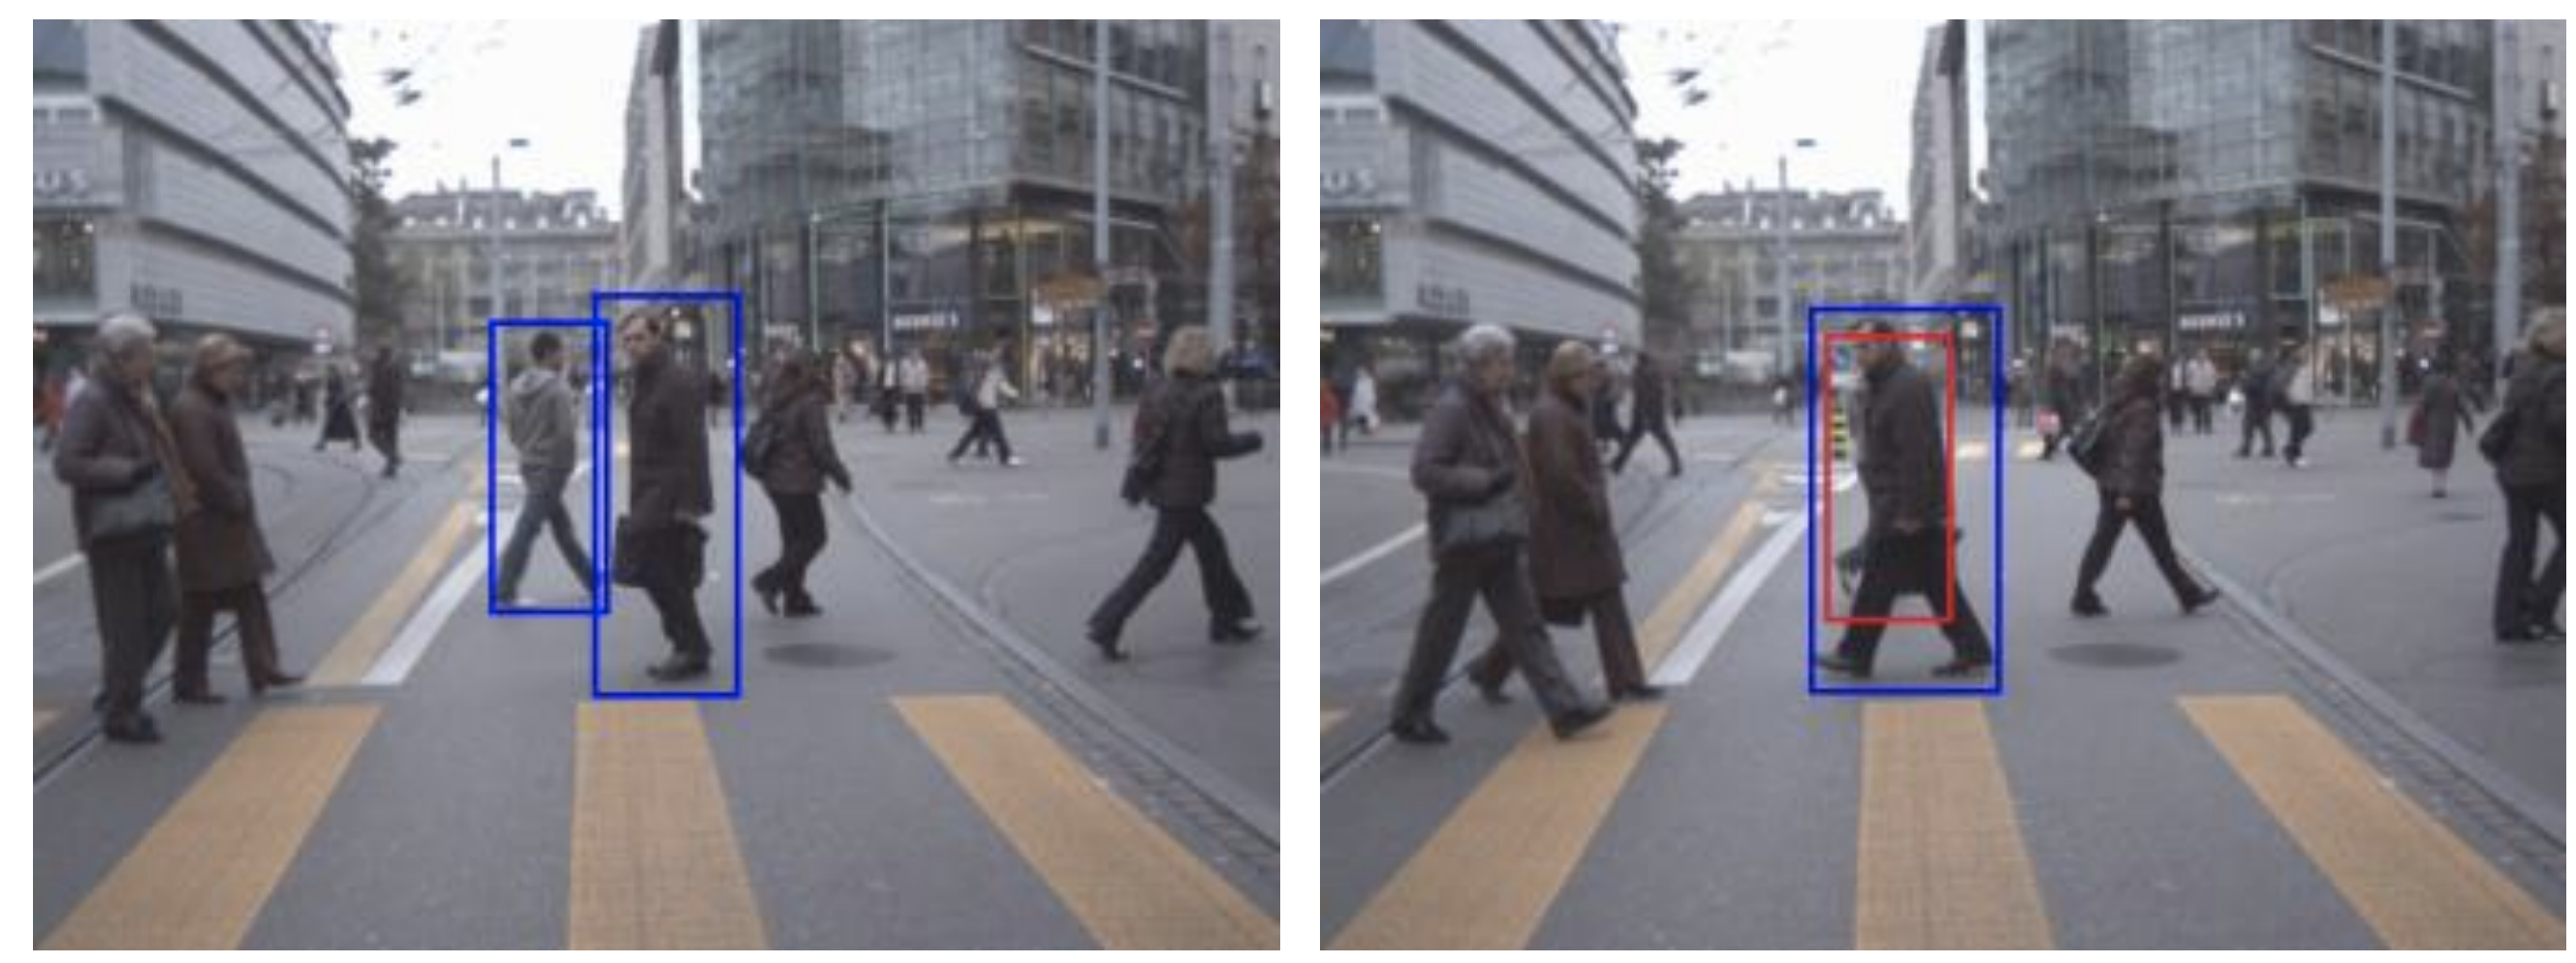
\includegraphics[width=0.9\textwidth]{figs/1-1/tbd.png}
	\caption{Tracking-by-detection~\cite{Breitenstein2010Online}示意图。蓝色框内为检测结果,红色框内为预测的匹配结果。}
	\label{fig:tracking_by_detection}
\end{figure}

大部分前景初始化的实现方法使用tracking-by-detection结构\cite{Breitenstein2010Online, Lee2014Driving},如图\ref{fig:tracking_by_detection}所示。Wangsiripitak等人\cite{Wangsiripitak2009Avoiding}假设对于一个三维物体,它的动态特征的位置是已知的。他们用边上的控制点集建模一个三维多面体模型,然后使用Harris’s RaPid tracker\cite{Harris1990RAPID}对其进行跟踪。如果之前跟踪的特征位于跟踪中的三维多面体上,当检测到这个物体处于移动状态时,便将特征剔除。被这个物体遮挡的静态特征也会被剔除。相似地,Wang等人\cite{Wang2010Visual}假设移动中的物体上的SURF特征描述子\cite{Bay2008Speeded}是已知的并存在数据库中。通过比较在特征检测步骤得到的描述子,就可以识别移动中的物体,也可以估算它的位移和旋转。Chhaya等人\cite{Chhaya2016Monocular}使用deformable wireframe object class model对建模相机前方的车辆。这个模型使用Principal Component Analysis (PCA) 在3D CAD data上训练而得。这个模型用在位姿估计得过程将车子识别并分割出来。另一方面,Lee等人\cite{Lee2014Driving, Lee2016Ground}基于tracking-by-detection结构,他们使用Constrained Multiple-Kernel(CMK)法,利用深度信息处理跟踪过程中的遮挡问题,同时使用预训练的人类检测器来跟踪行人。

有别于初始化前景的物体,背景初始化采用背景提取(background subtraction)技术 \cite{Babaee2017A,Piccardi2005Background}, 如图\ref{}所示。Zhang等人\cite{Zhang2012Visual}初始化属于背景的特征点集合,并令这个集合为背景的模型。他们假设当首次进行视觉的初始化时,是没有前景物体的。当经过新的一帧后,使用GPCA\cite{Ren2005Generalized}进行三维动态分割。分割出来的动态部分,对于先前的背景模型具有最高响应值部分,将会用来更新背景。根据新的背景模型,运用标准的对极几何法估计位姿。

\begin{figure}[thbp]
	\centering
	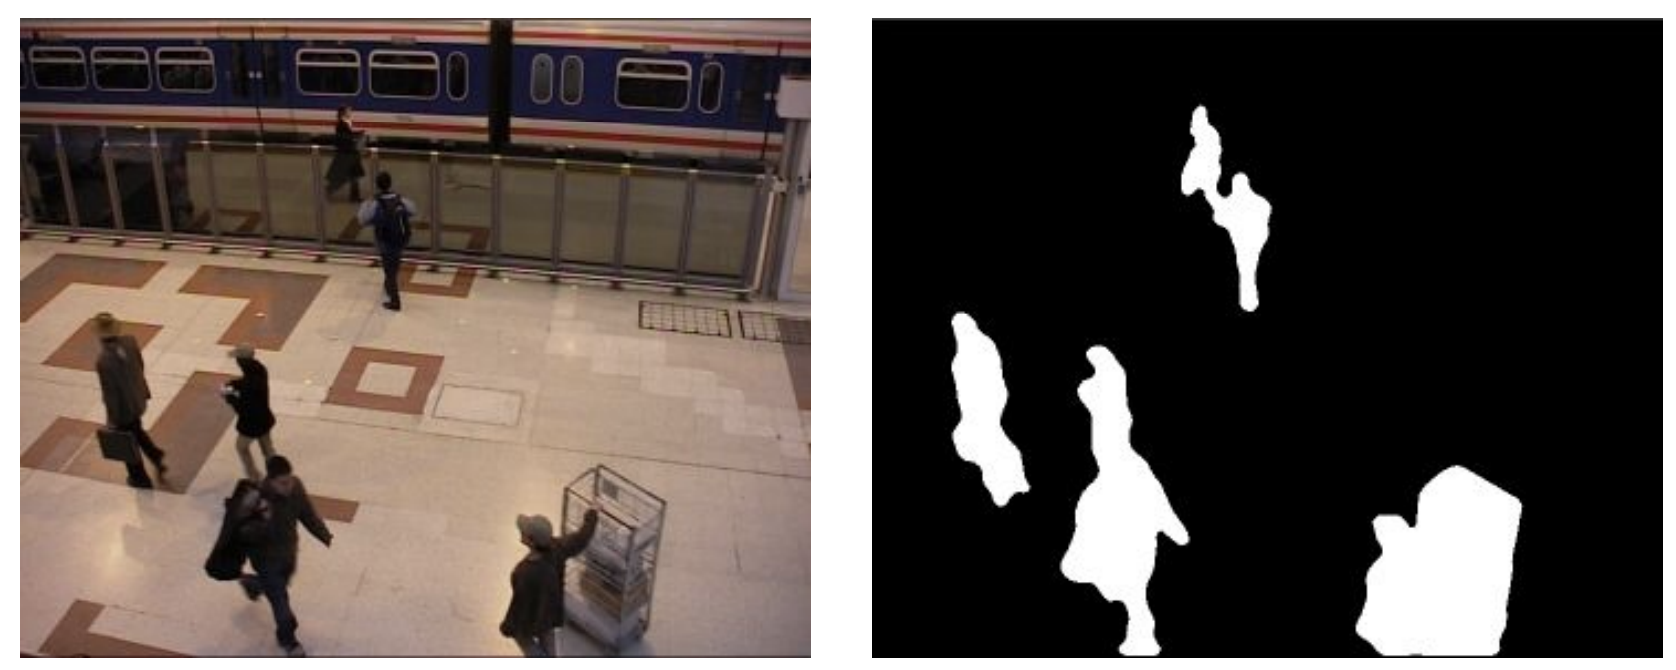
\includegraphics[width=0.9\textwidth]{figs/1-1/subback.png}
	\caption{基于~\cite{Babaee2017A}的背景提取结果。}
	\label{fig:tracking_by_detection}
\end{figure}

\subsubsection{基于几何约束的运动分割}
由于动态的特征会违反静态场景中的多视角几何约束,依赖此约束的技术是利用极限几何的性质\cite{Hartley2008Multiple}来分割静态和动态特征。这些约束可以从极线、三角化、基本矩阵估计或重投影误差的等式中得出。


Kundu等人\cite{kundu2009movingA}根据机器人里程计构建一个基本矩阵来定义两个几何约束。第一个约束是极线几何约束,在随后的视角下,成功匹配的点应该要在对应的极线上。如果跟踪到的特征离极线过远,就会被认为是动态特征。第二个约束是Flow Vector Bound(FVB),目的是分割当三维点沿着极线移动时产生的退化运动。通过设定跟踪到的特征流的上界和下界,超过这个范围的特征就会被作为运动的特征检测出来。最后通过循环的贝叶斯滤波器决定将特征分类为静态特征或动态特征。不同于使用极线约束,Migliore等人\cite{Migliore2009Use}利用三角化的原理分割静态和动态特征。他们在概率滤波器的框架下,持续地检查三个不同视角投影出来的视线的交点。如果特征是动态的,则这个交点在运动的过程中不会一样,甚至不会产生交点。但是由于传感器存在的噪声,他们使用Uncertain Projective Geometry\cite{Heuel2001Matching},将测量的不确定性加入他们检查不同视线关系的过程。最后通过统计方式分类静态和动态的特征。

将移动的物体误分类为静态物体并将其加入位姿估计,将会严重地使SLAM系统的性能降低,Lin等人\cite{Wang2007Simultaneous}通过观察这一性质来检测移动中的物体。他们计算两种不同条件下的位姿估计之间的差异,其中一个不加入新检测到的特征,另外一个假设新检测到的特征是静态的并加入位姿估计。借由计算两个结果的距离,设定一个门槛,通过二分贝叶斯滤波器整合,就能够精确地分割静态和动态的特征。

另外一个几何的方法是利用重投影误差。Zou和Tan\cite{Danping2013CoSLAM}将先前帧的特征投影到当前帧上,测量这些跟踪到到特征的距离。通过这个重投影的距离分类静态和动态的特征。Tan等人\cite{Wei2013Robust}使用同样的投影原理检测动态特征。他们同时将遮挡问题作为考量提出了一个鲁棒的视觉SLAM。在一个特征投影到当前帧上时,他们检测图像上的外观差异,也就是图像中的某一部分是否改变了。如果外观差异巨大,有极大的可能这个区域被动态物体遮挡,或是因为视点改变被静态物体所遮挡。因为上述原因被遮挡的三维点,会被保留并用来估算相机位姿。

\subsection{基于光流的运动分割}
光流的定义了两个连续的图像间,图案亮度的表面运动\cite{Horn1980Determining}。通常它对应了图像的运动场,因此可以用于分割移动的物体。Klappstein\cite{Klappstein2008Moving}根据光流定义了运动度量描述移动中的物体的似然。测量当场景中有运动物体时,光流错误的范围。Graph-cut算法根据运动度量分割移动的物体。

Alcantarilla等人\cite{Alcantarilla2012On}通过运动似然残差得到的场景流(三维的光流)中的三维运动向量系数,分割移动物体。马氏距离用于考量基于稠密光流和双目重建计算场景流的测量不确定性。如果残差小,特征点很可能属于静态物体。在运动似然残差设立门槛,属于运动物体的特征点可以从SLAM过程中删除,使得视觉里程计的估计更鲁棒。Derome等人\cite{Derome2015Moving, Derome2014Real}计算预测的预想与双目相机观测得到的图像的残差,以此计算光流。预测的图像是根据估计的相机自身运动,将当前帧的双目图像转换到过去的帧上。接着从残差场上的斑点检测移动中的物体。

\subsubsection{相机运动约束}
一般的SfM和视觉SLAM通过8点的均值\cite{Longuet1981A}或5点法\cite{David2004An}计算相机的运动。这种普通的相机运动估计并没有考虑任何相机移动方式的假设。另外一种方式是假设相机根据特定参数提供的外在信息(如车轮里程计的信息)估计相机位姿。加入这种相机运动约束,通过匹配特征点是否符合相机运动的约束,分类静态特征。

Scaramuzza\cite{scaramuzza20111A}提出利用轮式车辆的非完整性约束计算相机运动的方法。他假设相机运动是平面或圆形的,以此建模相机运动。由此约束,相机运动可以被参数化为1自由度并且可由1点法计算\cite{scaramuzza2009realA}。同样地,Sabzevari等人\cite{sabzevari2016multiA}也利用阿克曼转向几何提供的轮式车辆约束来计算相机运动。满足估计的相机运动的特征点会被认为是静态特征,其他的特征点则被认为是动态特征。

\subsubsection{运动分割的深度学习}
Lin和Wang\cite{Lin2014Deep}构建了一个可以显式地在图像空间分割移动物体的网络,他们使用Reconstruction Independent Component Analysis(RICA)自编码器\cite{NIPS2011_4467,Le2013Building}来学习时空特征,但是由于时空特征无法学习运动的三维几何信息,因此仍然使用几何特征帮助分割任务。几何特征和时空特征都放进循环神经网络(RNNs)来计算最终的运动分割。Fragkiadaki等人\cite{Fragkiadaki2015Learning}将RGB图像和光流的置信度\pjnote{objectness score??}。类似于AlexNet\cite{Krizhevsky2012ImageNet}的两个并行网络用来处理RGB图像和光流,接着放入回归网络生成运动估计\pjnote{motion proposal}。Valipour等人\cite{Valipour2017Recurrent}提出了Recurrent Fully Convolutioal Network(R-FCN),使用时序数据在线地在图像序列分割前景物体。Fully Convolutional Network(FCN)\cite{2014arXiv1411}用于学习空间特征和生成像素的稠密预测,但是Gated Recurrent Unit(GRU)用于在反卷积之前对时间特征进行建模。

\subsection{基于动态物体跟踪的SLAM技术}
\label{subsec:object_tracking}
动态物体分割和3D跟踪技术基于运动关系,将场景中的特征对应聚类成不同类别,并跟踪它们的三维轨迹。现有的动态物体分割技术可分为基于特征和基于深度学习的方法。其中,基于特征的方法的输入为场景中的所有特征或仅有动态物体的特征,基于深度学习的方法则可直接以图像作为输入,分割出动态物体。分割后的动态物体经过3D跟踪模块,输出动态物体的三维轨迹。另外,相机位姿和三维点云也可帮助动态物体的跟踪过程。本节将讨论分割和跟踪动态物体的相关技术研究。

\subsubsection{动态物体分割}
动态对象分割(也称为multi-body segmentation或eorumotion segmentation)将图像中的所有特征对应关系聚类成$n$个不同的运动类别。由于该问题是一个鸡生蛋、蛋生鸡的问题(chicken-egg problem),因此求解较为困难。为估计动态物体的运动,应首先对特征进行聚类;另一方面,聚类特征需要知道所有运动物体的运动模型。由于遮挡、运动模糊和特征跟踪丢失而带来的噪声、异常值和特征对应缺失使问题变得更加复杂。另一个挑战是如何处理退化运动(如当物体与相机在相同平面上以相同方向和速度移动)或相关运动(例如两个人一起移动,关节运动)的场景。本节讨论处理该类问题的现有方法。

\paragraph{静态模型选择}
在静态场景中,可通过一个运动模型来描述相邻帧特征点的对应关系。相反,动态场景中的特征点可能来源于具有不同运动模型的物体。运动模型通常基于以下几种模型:基础矩阵($F$),仿射基本矩阵($F_A$),本质矩阵($E$),单应性/投射($H$)或仿射($A$)矩阵。选择模型时,通常会尝试将所有可能的运动模型与数据拟合,并选择最适合数据的模型。如果数据可以由动态场景中的多个模型描述,则基于这些运动模型,需要建立许多假设才能进行动态物体的分割。

基于统计的3D动态物体分割方法会对数据的子集进行采样,并通过RANSAC~\cite{fischler1981randomA}或Monte-Carlo采样迭代~\cite{schindler2006two}用模型进行数据拟合。该类方法使用运动模型将数据划分为局内点(inlier,即符合该运动模型的数据)和局外点(outlier,不符合该运动模型的数据)。之后,对剩余的数据(即当前模型对应的局外点)再次采样,用新采样的数据拟合另一个运动模型,实现动静物体分割。该过程迭代重复,直到所有数据都可以由$n$个运动模型描述,或者剩余的异常值不足以产生更多的运动模型。迭代收敛后,该运动分割过程可从头开始,以生成许多候选的运动分割假设供后续选择。

目前,学者们已提出许多基于统计模型选择的方法来实现动态物体分割。Torr~\cite{faugeras1998geometric}对邻近的特征对应进行采样,并在RANSAC迭代下计算不同的运动模型($F, F_A, H, A$)。该方法用GRIC选择最能符合聚类局内点的运动模型。然而,当所选模型的局内点数量低于阈值时,则使用EM算法(expectation maximization)。为避免费时费力的暴力计算,Schindler和Suter~\cite{schindler2005two}~\cite{schindler2006two}提出了局部蒙特卡罗采样法,从图像上定义的子区域中进行采样。他们提出了一种从数据中估计噪声大小(noise scale)的方法,从而可以恢复每个运动的残差分布及其标准差。此外,他们推导出了一个新的似然函数,允许运动模型($F, H$)重叠,由GRIC选择最佳模型。

虽然之前的方法是对两个图像序列进行操作,但Schindler等人~\cite{schindler2006perspective}将~\cite{schindler2005two}中的技术扩展到一般运动模型(本质矩阵$E$)下的多视角图像。为了从多于两张图像的序列中将若干被选的本质矩阵关联起来,他们通过仅连接那些具有相似内点集的基本矩阵,来加强时间一致性。最后,使用类似MDL的方法来选择描述运动的最佳模型。这种方法已被Schindler等人泛化为适用于任何相机模型(不仅是投影相机)和运动模型(不仅是基本矩阵$E$)的动态物体分割方法~\cite{schindler2008model}。另外,Ozden等人也考虑了许多实际因素~\cite{ozden2010multibody},他们研究了如何将之前识别出的动态物体与静态背景融合,或如何将聚类分成两类不同运动模式的问题。

Thakoor等人~\cite{thakoor2010multibody}将模型选择描述为组合优化问题。采用branch-and-bound技术,通过将优化问题分解为较小的子问题,使用AIC作为代价函数来优化运动分割。对对应关系的局部采样也用于生成运动模式,而空假设(null hypothesis)用于处理局外点。最近,Sabzevari和Scaramuzza~\cite{sabzevari2014monocular}利用了基于投影轨迹矩阵分解的统计模型选择技术,通过对极几何生成运动模型,用重投影误差剔除不合理的假设。通过一次次迭代时不断优化结构估计和运动分割估计后,评估当前假设的合理性。该方法已在~\cite{sabzevari2016multiA}中得到拓展,通过施加相机位姿约束,相机和动态物体的位姿可以分别用单点法(one-point algorithm)~\cite{scaramuzza20111A}~\cite{scaramuzza2009realA}和两点法(two-point algorithm)~\cite{ortin2001indoor}求得。


\paragraph{子空间聚类}
子空间聚类是基于以下观察而被提出的:许多高维数据可以由低维子空间的并集来表示。数据点的子空间可以表示成基向量和数据的低维表示。子空间聚类框架下的三维运动分割问题基本可描述为找到与每个物体运动相关的子空间,并将数据拟合到子空间中。然而,由于在实际中子空间和数据分割是未知的,因此只能同时进行子空间参数估计和数据的子空间聚类。Costeira-Kanade~\cite{costeira1998multibody}和Gear~\cite{gear1998multibody}通过观察发现独立的刚体运动位于线性子空间中,从而首次提出了用子空间聚类进行运动分割的方法。通过施加秩(rank)的约束,可以恢复每一个线性子空间。

Kanatani~\cite{kanatani2001motionA}提出“子空间分离”的概念,将其作为聚类低维子空间的一般方法(不仅限于运动分割),借用统计模型选择实现子空间分离。该方法通过平衡在拟合数据点到子空间时残差的增加及子空间合并时自由度的减小,来选择最佳的子空间划分,并使用最小平方中值(least median of squares)法拟合带有局外点的数据。不同的是,Vidal等人~\cite{vidal2005generalized}扩展了主成分分析(principal component analysis)的概念,提出广义主成分分析(generalized principal component analysis, GPCA)法。PCA仅适用于数据都位于同一线性子空间内的情况,而GPCA可适用于数据位于多个线性子空间的情况。GPCA通过多项式嵌入(或Veronese映射)用$n$阶齐次多项式拟合数据,并通过计算特定点处多项式的导数找到每个子空间的法线,以解决寻找子空间的问题。然后,通过从法向量之间的角度计算相似性矩阵,使用谱聚类进行分割。为了在分割中考虑实际情况,在聚类前,该方法将数据投影到较低维空间中~\cite{vidal2005generalized},然后通过找到多项式嵌入的秩来计算运动模式的数量$n$。

由于之前的算法假设运动是刚性的,与实际情况还有一定差距,因此Yan和Pollefeys~\cite{yan2006general}提出了一个称为局部子空间仿射(local subspace affinity, LSA)的通用框架,可用于独立、铰接、刚性、非刚性、退化以及非退化的运动模式。LSA通过对点及其最近邻的区域进行采样,用局部子空间拟合采样数据,来估计子空间。最近邻的点可通过计算矢量之间的角度或距离得到。然后,通过计算两个局部子空间的夹角求解仿射矩阵,并对仿射矩阵进行谱聚类得到聚类结果。在估计子空间之前,还要将数据向低维子空间投影。与LSA类似,Goh和Vidal~\cite{goh2007segmenting}也用一个点及其最近邻点拟合局部子空间。基于局部线性嵌入法(locally linear embedding, LLE)~\cite{saul2003think},学者们提出了局部线性流形聚类法(locally linear manifold clustering, LLMC)。该方法使用LLE将数据转换为低维表示,并计算由LLE生成矩阵的零空间(null space)来将与每个运动相关联的分离的流形进行聚类,而其中数据的分离可由零空间中的向量表示。

Elhamifar和Vidal~\cite{elhamifar2009sparse}~\cite{elhamifar2013sparse}给出了另一种观点,它利用稀疏表示将运动模式进行聚类。他们发现线性或仿射子空间的并集中的点可以表示为子空间中所有数据点的线性或仿射组合,并提出了稀疏子空间聚类法(sparse subspace clustering, SSC)。然而,只有当点可被表示为同一子空间中数据的线性或仿射组合时,才能获得稀疏表示。在无噪声数据下,可以通过求解$L_1$最小化问题来估计稀疏系数。给定稀疏系数,可以构建仿射矩阵,通过谱聚类来完成聚类。Rao等人开发了SSC的扩展方法~\cite{rao2009motion},它们融合了稀疏表示和数据压缩以处理实际问题,例如数据丢失,不完整或包含局外点。最近,Yang等人~\cite{yang2015sparse}提出了矩阵补全技术来改进SSC算法。与稀疏表示相反,Liu~\cite{liu2012robust}和Chen等人~\cite{liu2010robust}采用低秩表示(low rank representation, LRR),使用谱聚类来定义仿射矩阵,实现子空间分割。

值得注意的是,大多数子空间聚类技术以批(batch)处理的形式进行。Vidal~\cite{vidal2007online}设计了一种迭代聚类技术,适用于位于多个移动超平面中的数据。该方法用一组时变多项式模拟了一组移动超平面,利用梯度下降,通过估计超平面的归一化法向量来递归地完成分割。Zhang等人提出了在线子空间聚类的另一种实现方式~\cite{zhang2009median}。他们修改了K-flats算法,使其能够增量地获取输入数据。他们将$L_1$用作目标函数(而非$L_2$),以便在数据包含噪声和局外点的情况下增强算法的鲁棒性。

在过去的几十年中,子空间聚类已经成为被广泛研究的课题,并且出现了许多方法。有关子空间聚类更详细的介绍,可阅读文献~\cite{vidal2011subspace}。

\subsubsection{动态物体的3D跟踪}
在实际应用中,跟踪三维空间中的动态物体并估计其三维坐标和深度具有非常重要的意义。该问题的挑战在于,一般的视觉SLAM系统假设场景是刚性、完全静止的,并用三角化方法~\cite{hartley1997triangulation}估计场景的三维结构,但该方法并不适用于动态物体,因为特征点重投影之后并不重合。假设$x_1$和$x_2$分别为第一帧和第二张帧图像中对应的特征点,则它们对应的3D点$X$的坐标应该能通过经相机投影矩阵$P_1$和$P_2$,计算$x_1$和$x_2$重投影光线的交点得到。但是,由于动态物体的运动和相机不同,因此从第一帧到第二帧重投影的光线也在移动,因此二者不相交。为解决动态物体的3D跟踪问题,需要其他的技术作为辅助。本节主要讨论估计动态物体的3D轨迹的相关工作。

\paragraph{轨迹三角化测量}
由前面的论述可知,标准的三角化测量~\cite{hartley1997triangulation}不能用于重建动态物体的3D结构,因为重投影的光线不相交。Avidan和Shashua~\cite{avidan1999trajectory}~\cite{avidan2000trajectory}提出了轨迹三角化测量方法,可在目标轨迹已知或满足某种参数形式的前提下,重建动态物体的三维点云。该方法假设3D点沿着三维空间中一条未知的直线运动,于是该问题就变成了寻找一条直线,与$t$个视角的投影光线都相交的问题。在$t$至少为5时,该问题有唯一解。因为3个视角的投影光线交叉将形成二次曲面,第4个视角的投影光线与该二次曲面交于2点,此时而第5个视角的投影光线便可使交点唯一确定。

与之相反,Shashua等人~\cite{shashua1999trajectory}假设物体在圆锥截面上移动。在这种假设下,需要至少9个视角才能获得唯一解。如果已知圆锥曲线的类型(圆、椭圆等),则只需要至少7个视角即可。他们通过将圆锥方程拟合二维空间中的运动点,或通过最小化三维空间中估计圆锥半径的误差来解决该非线性优化问题。基于之前的相关工作,Kaminski和Teicher~\cite{kaminski2002general}~\cite{kaminski2004general}将轨迹三角化问题泛化为在投影空间中找到一个超曲面簇。这种多项式的表示形式将非线性轨迹估计问题转化为未知参数空间中的线性问题。另一方面,为了处理缺失的数据,Park等人~\cite{park20103d}将3D轨迹表示为轨迹基矢量的线性组合,这样就可以用最小二乘法鲁棒地估计三维点云的位置。他们还通过分析相机运动、图像点运动和轨迹基矢量之间的关系,提出了可重构性标准(reconstructability criteria)。由于可重构性与3D重建误差成反比,因此该标准可以准确地考察精确重建的可能性~\cite{park20153d}。

\paragraph{粒子滤波器}
由于可观测性问题(观察者与目标之间的距离无法观测得到),单目相机进行动态物体的3D跟踪可被视为仅可跟踪(bearing-only-tracking,BOT)问题。单目相机可以被视为一种BOT传感器,它只能提供动态物体上被跟踪特征点的方向信息(例如上一帧和当前帧中对应的特征相对相机中心的角度)。对于BOT问题,往往使用基于滤波的方法,因为它可建模相机和目标的位置和速度的不确定性,并且已得到广泛的研究~\cite{aidala1983utilization}~\cite{le1998bearings}。

Kundu等人~\cite{kundu2011realtime}采用粒子滤波器来估计动态物体的位置和速度,他们用瞬时匀速运动模型(instantaneous constant velocity motion model)建模未知运动,并用李代数(Lie algebra)参数化动态物体的刚体变换。在初始化时,用几何约束和流向量绑定(flow vector bound)对动态物体进行分割~\cite{kundu2009movingA}~\cite{kundu2010realtime},并且使粒子沿投影光线均匀分布。利用由静态场景的三维点云估计得到的地平面和允许的最大深度值来约束粒子的空间。之后,将每个粒子投影到当前帧,计算重投影误差(投影点和实际特征点位置的误差)来更新每个粒子的权重。由于较低误差或较高权重的粒子具有较高的重采样概率,因此它们集中于能够产生最小重投影误差的深度值周围。

